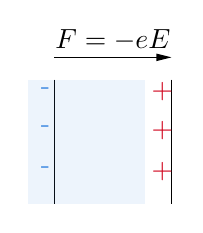
\begin{tikzpicture}[x=0.75pt,y=0.75pt,yscale=-0.6,xscale=0.6]
    %uncomment if require: \path (0,300); %set diagram left start at 0, and has height of 300
    
    %Straight Lines [id:da13477307007169825] 
    \draw    (100,123) -- (100,222.77) ;
    %Straight Lines [id:da43939624923609766] 
    \draw    (194,123) -- (194,222.77) ;
    %Shape: Rectangle [id:dp36771645669180764] 
    \draw  [draw opacity=0][fill={rgb, 255:red, 74; green, 144; blue, 226 }  ,fill opacity=0.1 ] (79,123) -- (173,123) -- (173,222.77) -- (79,222.77) -- cycle ;
    %Straight Lines [id:da5706192518127118] 
    \draw    (100,105) -- (192,105) ;
    \draw [shift={(194,105)}, rotate = 180] [fill={rgb, 255:red, 0; green, 0; blue, 0 }  ][line width=0.08]  [draw opacity=0] (12,-3) -- (0,0) -- (12,3) -- cycle    ;
    
    % Text Node
    \draw (87,123) node [anchor=north west][inner sep=0.75pt]  [color={rgb, 255:red, 74; green, 144; blue, 226 }  ,opacity=1 ] [align=left] {\mbox{-}};
    % Text Node
    \draw (87,154) node [anchor=north west][inner sep=0.75pt]  [color={rgb, 255:red, 74; green, 144; blue, 226 }  ,opacity=1 ] [align=left] {\mbox{-}};
    % Text Node
    \draw (87,187) node [anchor=north west][inner sep=0.75pt]  [color={rgb, 255:red, 74; green, 144; blue, 226 }  ,opacity=1 ] [align=left] {\mbox{-}};
    % Text Node
    \draw (176,123) node [anchor=north west][inner sep=0.75pt]  [color={rgb, 255:red, 208; green, 2; blue, 27 }  ,opacity=1 ] [align=left] {+};
    % Text Node
    \draw (176,154) node [anchor=north west][inner sep=0.75pt]  [color={rgb, 255:red, 208; green, 2; blue, 27 }  ,opacity=1 ] [align=left] {+};
    % Text Node
    \draw (176,187) node [anchor=north west][inner sep=0.75pt]  [color={rgb, 255:red, 208; green, 2; blue, 27 }  ,opacity=1 ] [align=left] {+};
    % Text Node
    \draw (147,102) node [anchor=south] [inner sep=0.75pt]    {$\boldsymbol{F} =-e\boldsymbol{E}$};
    
    
    \end{tikzpicture}
    